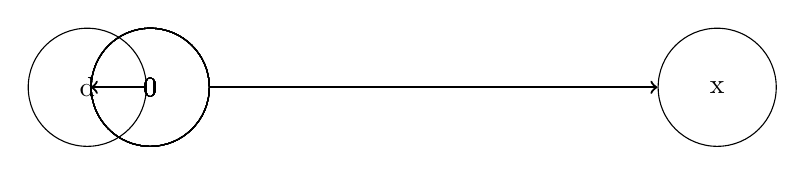
\begin{tikzpicture}[scale=0.2, every node/.style={draw=black,circle,inner sep=0pt}]
    \node [minimum size=1.5cm] (d) at (0,0) {d}; 
    \node [minimum size=1.5cm] (x) at (40,0) {x};                                    
    \node [minimum size=1.5cm] (0) at (4,0) {0};                                    
    \node [minimum size=1.5cm] (0) at (4,0) {0};                                    
    \node [minimum size=1.5cm] (0) at (4,0) {0};                                    
    \node [minimum size=1.5cm] (0) at (4,0) {0};                                    
    \node [minimum size=1.5cm] (0) at (4,0) {0};                                    
    \node [minimum size=1.5cm] (0) at (4,0) {0};                                    
    \node [minimum size=1.5cm] (0) at (4,0) {0};                                    
    \node [minimum size=1.5cm] (0) at (4,0) {0};                                    
    \node [minimum size=1.5cm] (0) at (4,0) {0};                                    
    \node [minimum size=1.5cm] (0) at (4,0) {0};                                    
    \draw [thick, ->] (d) -- (0);                                 
    \draw [thick, ->] (0) -- (x);                                 
\end{tikzpicture}                                                       